% Rendered from proposal.md (same text). Build: xelatex proposal.tex
\documentclass{article}
\usepackage[letterpaper,margin=0.55in,top=0.5in,bottom=0.5in]{geometry}
\usepackage{fontspec}
\setmainfont{Times New Roman}
\usepackage{graphicx,booktabs,tabularx,enumitem,xcolor}
\usepackage{xurl}
\usepackage[hidelinks]{hyperref}
\usepackage[compact]{titlesec}
\titleformat{\section}{\normalfont\bfseries\large}{\thesection.}{0.4em}{}
\titlespacing*{\section}{0pt}{5pt}{2pt}
\setlist{nosep,leftmargin=1.2em}
\setlength{\parindent}{0pt}
\setlength{\parskip}{3pt}
\pagestyle{empty}
\begin{document}
\fontsize{10.5pt}{12.4pt}\selectfont

{\centering
{\Large\bfseries Teaching Aerial Imagery to See Height: Tracking Philadelphia's Gentle Densification with LiDAR-Supervised Foundation Models\par}
\vspace{3pt}
Xuanyu Zhou · AI Urban Sustainability · Final Project Proposal\par}

\section{Background and Research Questions}
Adding homes inside the existing city is one of the most sustainable ways to grow. Infill and vertical additions use existing streets, transit and utilities, avoid greenfield development, and cut per-capita travel and energy use. Philadelphia's rowhouse neighborhoods densify one lot at a time: vacant lots are filled with new rowhouses, and existing homes gain an extra story (``pop-ups''). Pop-ups are contested enough that City Council has capped them in parts of the city; for example, Bill No.~230574 (2023) limits residential height in Brewerytown--Sharswood to that of the tallest abutting building [3]. Yet the city has no consistent, building-level record of \emph{where} and \emph{when} the built fabric grows. Permits record intent, not outcomes.

Airborne LiDAR measures building height directly, but Philadelphia flies it only every three to four years (most recently 2018, 2022 and 2025). Aerial imagery is flown every spring but contains no height. In Meta and WRI's Canopy Height Maps v2, a DINOv3 backbone pretrained on satellite imagery and supervised by LiDAR raised $R^2$ for tree height from 0.53 to 0.86 [1,\,2]. We use the three LiDAR flights as measured anchors and train a model that, starting from the last flight, reads from each year's imagery which parcels have grown since then.

\textbf{Scope.} Residential and low/mid-density mixed-use zoning: 152.5\,km$^2$ of current base districts. The high-rise core (CMX-4/5), industrial and special-purpose districts and the Navy Yard are excluded.
\begin{itemize}
\item \textbf{RQ1 (AI):} How far can a LiDAR-anchored, bi-temporal DINOv3 model track new construction and vertical additions from aerial imagery in unseen places and years, and at what spatial scale are its results reliable?
\item \textbf{RQ2 (Urban):} Where, how much and \emph{when} did Philadelphia densify through infill and vertical additions between 2018 and 2025, relative to transit access and neighborhood socioeconomic change?
\item \textbf{RQ3 (Governance):} What share of building permits results in visible construction, how long does it take, and how much change happens without a matching permit?
\end{itemize}

\section{Data}
\begin{tabularx}{\linewidth}{@{}>{\raggedright}p{0.38\linewidth}>{\raggedright}X>{\raggedright\arraybackslash}p{0.2\linewidth}@{}}
\toprule
Data & Years & Role\\ \midrule
City LiDAR point clouds (PASDA) & Anchors 2018, 2022, 2025 (15--50 pts/m$^2$); 2010 and 2015 (sparse) for extra training pairs & Height, change labels, anchors\\
City aerial orthoimagery (3-inch; April--May) & 2018, 2019, 2020, 2022, 2023, 2024, 2025 & Model input\\
L\&I building permits (OpenDataPhilly / Carto) & 2014--2025 & Validation, RQ3\\
Zoning base districts (current), parcels (2016, 2025), footprints (2017), ACS 5-year, SEPTA stops & -- & Study area, analysis units, RQ2 context\\ \bottomrule
\end{tabularx}

The 2025 flight was on \textbf{18 April 2025} according to the point timestamps. PASDA's metadata gives ``April 2022'', which is copied from the earlier flight.

\section{AI Methods}
\textbf{LiDAR change detection.} Per parcel, 0.5\,m normalized surface models from each flight, vegetation removed by multi-return structure (and point classes in 2025, flown as leaves emerged), rule-based classes: new construction, vertical addition, rear extension, demolition. In anchor years, vertical additions are measured directly by LiDAR.

\textbf{LiDAR-anchored bi-temporal model.} DINOv3 ViT-L/16 pretrained on satellite imagery (SAT-493M) encodes the anchor-year image and the current image. A DPT-style head fuses both with the anchor-year LiDAR height. Features are pooled per parcel unit, and two heads score whether the unit \emph{grew} and whether it is a \emph{vertical addition}; a height-change regression is an auxiliary loss. The model dates changes in the years between flights (2019, 2020, 2023, 2024). Parcel-level counts are calibrated to grid cells with validation precision and recall. Earlier variants were tested and dropped: a single-image height model, two-image change regression, and anchored height regression.

\textbf{Evaluation and next steps.} Every split is held out in space, and the final tests also in time. Decision rules are written down before results are seen. The training area is being expanded citywide to test whether vertical additions are limited by sample size. Second round: retrain on the citywide split and test \textbf{once} on 8 newly sealed ZIP codes (2022$\to$2025), stratified by rowhouse, detached and mixed areas.

\section{Pilot Results}
\begin{tabularx}{\linewidth}{@{}>{\raggedright}p{0.3\linewidth}>{\raggedright\arraybackslash}X@{}}
\toprule
Test & Result\\ \midrule
LiDAR change detection (19146, 2018$\to$2022) & Recall: \textbf{96.6\%} of new-construction permits ($n=417$), \textbf{87.1\%} of vertical-addition permits ($n=93$). Precision on a fresh blind sample: \textbf{95.5\%} (42 of 44).\\
Single-image height model & Building-level MAE 1.17--1.60\,m; misses vertical additions (sees 1.9 of 3.8\,m)\\
Round-1 final test of the bi-temporal model (19146 + 19147, 2022$\to$2025, run once) & Grid-level correlation with LiDAR for \emph{grew} and \emph{new construction}: \textbf{0.83--0.88} at 250\,m and block group; totals within 10\%. Per-parcel vertical additions: AP only \textbf{0.16}, a known limitation.\\ \bottomrule
\end{tabularx}

Large structural changes in the pilot area were well covered by permits: every detected pop-up had a related permit, and only 4 changes were confirmed without one. The project therefore focuses on \emph{where and when densification happens}, not on enforcement.

\begin{center}
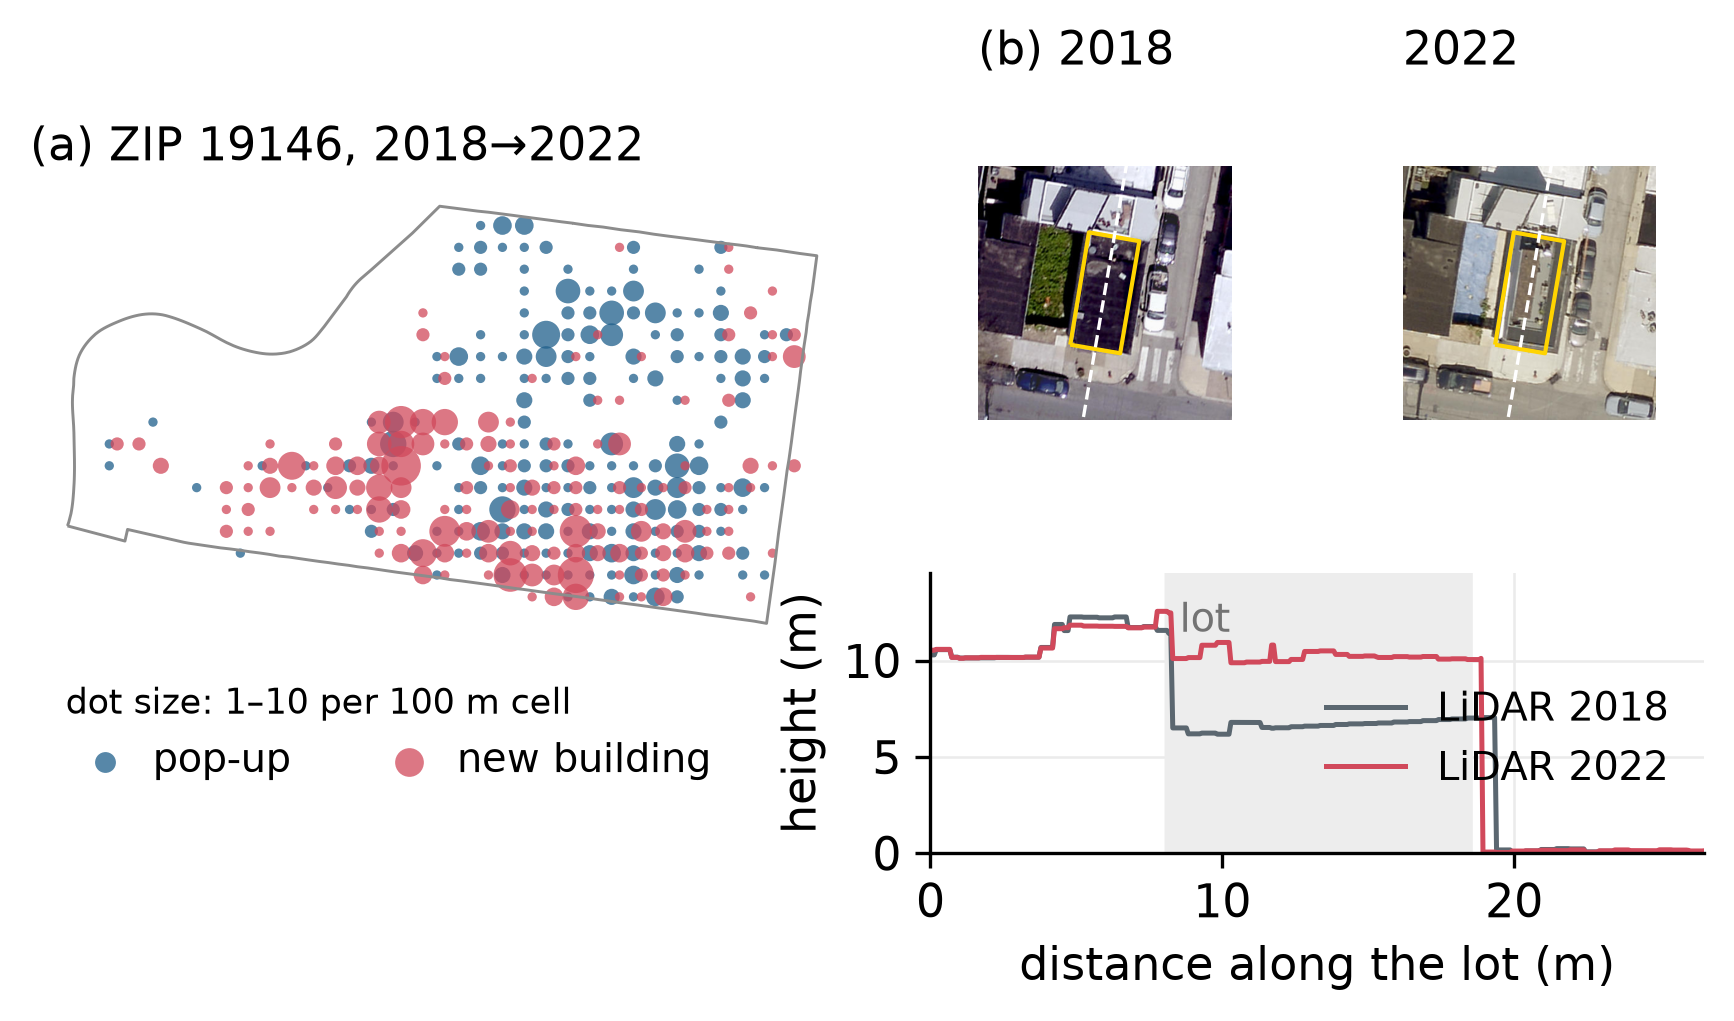
\includegraphics[width=0.6\linewidth]{fig1.png}\\[-2pt]
{\textbf{Figure 1.} (a) LiDAR-detected pop-ups and new construction per 100\,m cell, ZIP 19146, 2018$\to$2022. (b) A permitted pop-up: aerial images and the LiDAR height profile along the lot; the roof rose from about 6.5\,m to 10\,m.}
\end{center}

\section{Remaining Work and Expected Outcomes}
\begin{enumerate}
\item \textbf{Citywide model:} LiDAR (five years) and imagery (nine years) are processed over the study area; next, retrain on the citywide split and run the round-2 test.
\item \textbf{RQ2:} densification maps at 100\,m, 250\,m and block-group scale for 2018--2025, combining LiDAR anchor years with model-dated intermediate years. Growth is related to transit access and socioeconomic change.
\item \textbf{RQ3:} permit-to-construction rates and time to completion by neighborhood.
\item \textbf{Interactive map} of aggregated results; no address is labeled with permit status.
\end{enumerate}
\textbf{Limitation.} Vertical additions are reported from LiDAR anchor years unless the round-2 test shows grid-level correlation $\geq 0.8$.

\vspace{2pt}
{\textbf{References.}
[1] Meta AI \& World Resources Institute (2026). \emph{Canopy Height Maps v2.} \url{https://ai.meta.com/blog/world-resources-institute-dino-canopy-height-maps-v2/}
[2] Siméoni, O., et al. (2025). \emph{DINOv3.} arXiv:2508.10104.
[3] City of Philadelphia, Bill No.~230574 (2023), Brewerytown--Sharswood overlay; \emph{Philadelphia Inquirer}, 16 Nov 2023.
[4] Philadelphia L\&I permits and zoning base districts, OpenDataPhilly.
[5] PASDA, Philadelphia LiDAR and aerial photography, 2010--2025.\par}
\end{document}
